\documentclass[a4paper, 10pt, twocolumn]{article}
% Sowohl LaTeX als auch pdfLaTeX können benutzt werden, um das Manuskript zu erstellen.

% Bitte öffnen sie diese Datei mit utf8 Zeichenkodierung!!!
\usepackage[utf8]{inputenc}         % Schriftkodierung dieser Datei
\usepackage[german]{babel}          % für deutsche Dokumente

\usepackage{graphicx}               % optional für Grafiken
\usepackage{tabularx}               % optional für Tabellen
\usepackage{multirow}               % optional für Tabellen
\usepackage{url}                       % optional für Internet Links

\usepackage[small,bf]{caption2}     % bitte für Bildunterschriften verwenden
\usepackage{parskip}
\usepackage{titlesec}
\usepackage{amsmath}                % optional für Formeln


\titleformat{\section}{\normalfont\large\bfseries}{\thesection}{}{}
\titleformat{\subsection}{\normalfont\large\bfseries}{\thesection}{}{}
\titleformat{\paragraph}{\normalfont\bfseries}{\theparagraph}{}{}
\titlespacing{\section}{0pt}{6pt}{-1pt}
\titlespacing{\subsection}{0pt}{3pt}{-1pt}
\titlespacing{\paragraph}{0pt}{3pt}{-1pt}

\newcolumntype{Y}{>{\centering\arraybackslash}X}    %für Tabellen mit tabularx

% Definition der Seitenränder
\addtolength{\textwidth}{2.1cm}
\addtolength{\topmargin}{-2.4cm}
\addtolength{\oddsidemargin}{-1.1 cm}
\addtolength{\textheight}{4.5cm}
\setlength{\columnsep}{0.7cm}

\pagestyle{empty}                   % weder Kopf- noch Fußzeile auf 1. Seite

\begin{document}

\date{}                                         % kein Datum auf 1. Seite

\title{\vspace{-8mm}\textbf{\large
Vergleich der MIR Audio Features von Spotify mit subjektiven Einschätzungen }}

% Hier die Namen und Daten der beteiligten Autoren eintragen
\author{
Anyere Bendrien$^{1,2}$, Sebastian Cycon$^{1,3}$, Maximilian Wagenbach$^{1,4}$\\\
$^{1}$\emph{\small TU Berlin, Fachgebiet Audiokommunikation, 10623 Berlin, Deutschland} \\
$^{2}$\emph{\small anyere.bendrien@campus.tu-berlin.de},
$^{3}$\emph{\small cycon@campus.tu-berlin.de},
$^{4}$\emph{\small maxijuli@t-online.de} }
\maketitle
\thispagestyle{empty}           % weder Kopf- noch Fußzeile auf Folgeseiten

% Beginn des eigentlichen Manuskripts
\section*{Einleitung}
\label{sec:Einleitung}

Im Digitalen Zeitalter ist es immer wichtiger große Datenmengen zu untersuchen und speziell an Informationen über deren Inhalt zu gelangen.
Mit Hilfe verschiedener Techniken ist es möglich, vielfältige Informationen über den Inhalt von digitalen Daten zu extrahieren, wodurch sie sich für eine informationstechnische Weiterverarbeitung eigenen.
Die Entwicklung solcher Methoden für musikalische Inhalte allgemein ist Gegenstand des interdisziplinären Forschungsgebiets \textit{Music Information Retrieval}, kurz \textit{MIR}.
So ist es beispielsweise möglich, mit computergestützten Verfahren, grundlegende Metriken wie das Tempo, die Tonart oder das Tongeschlecht aus einem Musikstück zu extrahieren\,\cite{Casey2008}.
Aufbauend auf diesen Metriken lassen sich komplexere Attribute vorhersagen, welche subjektiven Empfindungen entsprechen\,\cite{Sturm2013}.
Als Beispiel wäre die Fröhlichkeit, die Tanzbarkeit oder die Komplexität eines Musikstücks zu nennen.
In diesem Kontext gewonnene Informationen werden auch \textit{Audio Features} genannt.
Unter anderem lassen sich Audio Features in Beziehung zueinander stellen, um so Zusammenhänge zwischen den zugrunde liegenden Daten ermitteln zu können.
So ist es beispielsweise möglich automatisch Playlisten für einen Nutzer zu erstellen oder dem Nutzer Musik vorzuschlagen, die er noch nicht besitzt, welche aber seinem Musikgeschmack entspricht.

%Das Streamen von medialen Inhalten über das Internet ist im gesellschaftlichen Alltag kaum noch wegzudenken. % kürzen?
Der On-Demand Streaming-Dienst \textit{Spotify}\footnote{Website: \url{https://www.spotify.com/}} hat sich auf Audiodaten spezialisiert.
Er stellt seinen Nutzern eine umfangreiche Sammlung von Musik zum Hören über das Internet zur Verfügung und wendet auf diesen Daten eigene \textit{MIR} Verfahren an.
\textit{Spotify} extrahiert aus der Musik \textit{Audio Features} und macht diese über eine Schnittstelle öffentlich abrufbar.
Aufbauend darauf ist eine Vielzahl an informationstechnischer Weiterverarbeitung möglich, für welche jedoch der Wahrheitsgehalt der abgerufenen Informationen einen großen Stellenwert hat.
Dies führt zu der schwer greifbaren und aktuellen Problematik im Feld des \textit{MIR}:
Wie lassen sich die Ergebnisse unterschiedlicher \textit{MIR} Verfahren und Algorithmen bewerten und mit einander vergleichen? \cite{Downie2004}

In der Praxis kommen verschiedene Evaluationsverfahren zum Einsatz.
Ein Verfahren mit Blick auf \textit{Gültigkeit}, \textit{Zuverlässigkeit} und \textit{Effizienz} \cite{Urbano_2013}, wird im Folgenden genauer beschrieben.
Durch \textit{MIR} extrahierte \textit{Audio Features} werden einer Aggregation von Vergleichsinformationen gegenübergestellt und mit ihr abgeglichen (\textit{Gültigkeit}), um eine Aussage über ihren Wahrheitsgehalt treffen zu können.
Damit die aggregierten Daten als Vergleichsmaß herangezogen werden können, muss zuvor sichergestellt werden, dass sie sowohl inhaltlich als auch quantitativ einem Mindestmaß an Qualität entsprechen (\textit{Zuverlässigkeit}).
Um die Validität dieser Vergleichsdaten sicher zu stellen werden diese häufig von Menschen bewertet.
Ein solcher Datensatz wird auch als \textit{ground truth} bezeichnet.
Unter \textit{Effizienz} versteht man die Wiederverwertbarkeit der ground truth Daten für verschiedene Studien und Forschergruppen.
Um nun die Qualität der Ergebnisse eines Algorithmus zu bewerten, werden diese mit den ground truth Daten verglichen.
Über den Grad der Korrelation zwischen den beiden Datensätze lassen sich Aussagen über die Ergebnisse von MIR Algorithmen treffen.

In dieser Studie werden die Audio Features von Spotify nach diesem Prinzip auf ihre Qualität geprüft.
Dazu werden sie ebenfalls mit einem von Menschen bewerteten Datensatz verglichen.
Dies führt uns zu folgender Hypothese:
Die von \textit{Spotify} bereitgestellten \textit{Audio Features} korrelieren mit einem Korrelationskoeffizienten von 0,5 oder mehr mit den subjektiven Bewertungen von Menschen.

\section*{Methoden}
\label{sec:Methoden}

Da es sich bei dieser Studie um eine Zweitverwertung des Datensatzes einer anderen Studie handelt mussten die Daten zunächst für diese Studie neu strukturiert und angepasst werden.
Der verwendete Datensatz stammt aus einer Studie, in der die Probanden angeben sollten welche 10 Songs sie mit auf eine einsame Insel nehmen würden. [ PAPER LINK ]
Anschließend mussten sie zu den von ihnen gewählten Songs 13 verschiedene Attribute, wie zum Beispiel Entspannend, Komplex, Tanzbar oder Traurig, bewerten.

Der Datensatz enthielt 45 Datenpunkte in denen sich je ein Proband mit seinen 10 Songs und deren Bewertungen befindet.
Ein Problem, das sofort ins Auge fällt, ist, dass der Datensatz schwer maschinenlesbar ist. 
Zum Beispiel sind die Songtitel und der Interpret beliebig vermischt und folgten keinem klaren Schema.
Um eine Analyse der einzelnen Songs zu ermöglichen, mussten zunächst mit Hilfe eines Python Skripts aus dem bestehenden Datensatz die einzelnen Songs und deren Bewertungen extrahieren werden.
Anschließend wurden die Daten zu insgesamt 450 neuen Datenpunkten zusammengefasst, die jeweils einen Song und seine Bewertungen enthalten.
Zusätzlich wurde die Daten aus dem veralteten CSV Format in das deutlich einfacher maschinell lesbare JSON Format konvertiert.

Um die Spotify Audio Features für einen Song zu ermitteln muss der Spotify Programmierschnittstelle (API) die dem Song entsprechende Spotify ID übergeben werden.
Diese muss zunächst für jeden Song ermittelt werden.
Da die Songtitel und Interpreten maschinell nicht einfach und klar voneinander trennbar waren, wurde die Spotify Suchfunktion verwendet.
Dieser kann eine gemischte Zeichenkette mit Titel und Interpret übergeben werden.
Sie liefert daraufhin Informationen über die Treffer der gefundenen Songs in der Spotify Datenbank mitsamt der Spotify IDs.
Wir haben die ID des ersten gefunden Treffers zu dem entsprechenden Datenpunkt des bisherigen Datensatzes hinzugefügt.
Insgesamt 50 der Songs konnten entweder auf Grund der vermischten Sucheingabe oder weil sie nicht in der Spotify Datenbank vorhanden sind nicht gefunden werden.
\footnote{Der Zugriff erfolgte am 23.2.2017 gegen 16:00 Uhr.}
Auch dieser Schritt wurde mit einem Python Script automatisiert durchgeführt.
Dafür wurde die Spotipy \footnote{Spotipy Programmbibliothek: \url{https://github.com/plamere/spotipy}} Python Bibliothek verwendet, welche einen einfachen Zugriff auf die Spotify Web Schnittstellen ermöglicht.
Nach diesem Schritt enthielt der neuer Datensatz 400 Songs mit den Probandenbewertungen und der Spotify ID.

Bei der Durchsicht des Datensatzes fiel auf, dass es sich bei einige der von Spotify gefunden Ergebnisse um völlig andere Songs handelte.
Teilweise wurden auch Instrumental Versionen oder Cover Versionen der Songs gefunden.
Stichproben ergaben das die Original Versionen dieser Songs sich nicht in der Spotify Datenbank befinden.
Aus diesem Grund wurde im Anschluss eine Datenvalidierung durchgeführt.
Dabei wurde ein einfacher Stringvergleich zwischen dem Originaltitel des "`10 Songs für die einsame Insel"' Datensatz und einer Kombination aus dem von Spotify gefunden Titel und Interpreten durchgeführt.
Eine Ähnlichkeit der Zeichenketten von 60\% führte zu einem guten Kompromiss zwischen Genauigkeit und Freiheitsgrad.
Dadurch wurden aus dem Datensatz weitere 49 Einträge entfernt, was zu einer Gesamtanzahl von 351 Datenpunkten führte.

Als nächsten Schritt wurde mit Hilfe der Spotipy Bibliothek der Spotify Audio Feature Web API die ermittelten Spotify IDs übergeben.
Dafür muss man sich zunächst bei Spotify als Developer anmelden, um eine Autorisierung zu erhalten mit der man auf die Spotify Audio Feature Web API zugreifen kann.
Für jede angefragte ID liefert die Spotify Audio Feature Web API ein JSON Objekt\,\footnote{Dokumentation: \url{https://developer.spotify.com/web-api/get-audio-features/}} zurück.
Aus diesem haben wir die für diese Studie relevanten Audio Features extrahiert und in den entsprechenden Eintrag unseres Datensatzes eingefügt.
\footnote{Der Zugriff erfolgte am 23.2.2017 gegen 16:15 Uhr.}
Dieser Vorgang wurde entsprechend für alle 351 Datenpunkte durchgeführt.

Von den insgesamt 13 von Spotify zur Verfügung gestellten Audio Feature Attributen nur 8 verwendet.
Da die Bewertungen der Umfrage subjektiven Einschätzungen entsprechen, wurden die Attribute, welche die Struktur eines Musikstücks beschreiben, nicht in die statistische Analyse mit einbezogen.
Zu diesen Attributen gehören die Länge des Songs (``duration\_ms''),  die Taktangabe (``time\_signature'') sowie die Tonklasse (``key'').
Außerdem wird das Audio Feature ``mode'' (Tongeschlecht) nicht berücksichtigt, da es sich um eine dichotome Variable handelt, welches sich für das verwendete statistische Verfahren nicht eignet.
Die verwendeten Spotify Audio Features sind im folgenden kurz beschrieben:

\begin{description}
    \item[acousticness] Variable die beschreibt wie Wahrscheinlich es sich um einen Akustiksong handelt.
    \item[danceability] Zusammengesetzte Variable die beschreibt wie Tanzbar ein Song ist. Setzt sich aus verschiedenen musikalischen Elementen wie Tempo, Rhythmusstabilität, Beatstärke oder Regelmäßigkeit.
    \item[energy] Beschreibt die gefühlte Wahrnehmung von Intensität und Aktivität. Deathmetal hat beispielsweise eine hohe Energie, ein Bach Choral eine niedrige. Der Wert setzt sich unter anderem aus der Dynamik, der wahrgenommenen Lautstärke, der Klangfarbe, den Einsätzen und der generellen Entropie.
    \item[instrumentalness] Vorhersage darüber ob der Song keinen Gesang enthält.
    \item[liveness] Ermittelt die Anwesenheit eines Publikums. Je höher der Wert desto wahrscheinlicher wurde der Song Live aufgenommen.
    \item[loudness] Gemittelter Lautstärkewert des Songs in Dezibel (dB).
    \item[speechiness] Variable die angibt wie viel innerhalb eines Songs gesprochen wird. Hohe werte stehen für Podcasts oder Hörbücher, mittlere Werte stehen für Musik mit hohem Anteil an Sprache (wie zum Beispiel Rap) und niedrige Werte entsprechen Musik ohne Sprache.
    \item[tempo] Anzahl der Beats per Minute (Bpm).
    \item[valence] Maß für die musikalische Fröhlichkeit eines Songs. Songs mit einer hohen Valence werden als fröhlich und heiter empfunden. Songs mit einer niedigen Valence werden als traurig oder deprimierend wahrgenommen.
\end{description}

Da die weitere statistische Auswertung des Datensatzes in der SPSS Software geschah mussten die Daten anschließend vom JSON in das CSV Format konvertiert werden, da dieses das einzige Format ist das SPSS akzeptiert.

Der gesamte Code, der für die Aufbereitung der Daten geschrieben wurde, ist unter einer Open Source Lizenz auf GitHub.com veröffentlicht \footnote{Code Repository:\hfill \url{https://github.com/Bendrien/SpotifyMIR-Evaluation/tree/master/python}}.



\section*{Statistische Methoden}
\label{sec:Statistische Methoden}

Um zu Untersuchen ob und wie stark die von Probanden abgegebenen Bewertungen mit den von Spotify generierten Audio Features korrelieren, wurde eine Regression verwendet.
Nach der beschriebenen Vorbereitung des Datensatzes wurde zunächst eine Datenreduktion durchgeführt.
Mit Hilfe eine Faktorenanalyse soll so aus den 13 Attributen, die von den Probanden bewertet wurden, einige wenige Faktoren werden.
Dazu wurde eine Hauptkomponentenfaktorenanalyse mit orthogonaler Achsenrotation (Varimax Verfahren) verwendet.

Anschließend wurde eine multiple schrittweise Regression durchgeführt.
Die reduzierten Faktoren wurden dabei als abhängige Variable verwendet und die Attribute des Spotify Algorithmus als unabhängige Variablen.

\section*{Ergebnisse}
\label{sec:Ergebnisse}

Entsprechend dem Kaiser-Kriterium für signifikante Faktoren ab einem Eigenwert von mindestens 1 erstellt die Faktorenanalyse aus den 13 von Probanden bewerteten Attributen vier Faktoren.
Das Kaiser-Meyer-Olkin-Kriterium der Faktorenanalyse nimmt einen Wert von 0,734 an, was einem ziemlich guten Ausmaß an Interkorrelation zwischen den Variablen entspricht \cite{eckey2002multivariate}.
Die vier Faktoren decken insgesamt 67\% der Gesamtvarianz.
Wenige Variablen laden dabei mit einer Faktorladung von mindestens 0,66 relativ stark in einen Faktor, während sie gleichzeitig mit einem maximalen Wert von 0,46 eher schwach in die übrigen Faktoren laden.
Einzig die Variable \textit{Emotional} lädt in keines der Faktoren stark und entfällt aus diesem Grund aus der inhaltlichen Beschreibung der erzeugten Faktoren.
Die vier erzeugten Faktoren werden inhaltlich gekennzeichnet als \textit{Ruhig} für den 1. Faktor, \textit{Niveauvoll} für den 2. Faktor, \textit{Heiter} für den 3. Faktor und \textit{Energisch} für den 4. Faktor (vgl. Tabelle \ref{tab:faktoren}).   


\begin{table}[htbp]
    \centering
    \caption{Ergebnis der Faktorenanlyse}
    \vspace{2mm}
    \label{tab:faktoren}
        \begin{tabularx}{8.4cm}{@{\extracolsep{\fill}} @{\arrayrulewidth1.5pt\vline}Y@{\arrayrulewidth1.5pt\vline}Y@{\arrayrulewidth1.5pt\vline}}
            \noalign{\hrule height1.5pt}
            1. Faktor: \textbf{Ruhig} & 2. Faktor: \textbf{Niveauvoll} \\
            \hline
            Entspannend        & Anspruchsvoll \\
            Warm               & Komplex \\
            Sanft              & - Einfach \\           
                               & Intellektuell \\
            \noalign{\hrule height1.5pt}
            3. Faktor: \textbf{Heiter} & 4. Faktor: \textbf{Energisch} \\
            \hline
            Fröhlich             & Erregend \\
            - Traurig            & Intensiv \\
            Tanzbar              & \\
            \noalign{\hrule height1.5pt}
        \end{tabularx}
\end{table}


Die Regressionen dieser Faktoren mit den Features von Spotify liefern Modelle mit sehr hohen Signifikanzen nahe 0 (vgl. Tabelle 1).
Als Kriterium für das Aufnehmen einer Variable für ein Modell ist ein maximaler Signikanzwert von  0,05.  
Das Modell mit der höchsten Güte erhalten wir bei der Regression mit dem Faktor \textit{Heiter}.
23,1\% der Varianz wird vom Modell, dass die Variablen \textit{SP\_danceability}, \textit{SP\_energy}, \textit{SP\_instrumentalness} und \textit{SP\_valence} enthält, gedeckt.
Die Variable \textit{SP\_energy} ist in dem Modell am stärksten gewichtet, gefolgt von den Variablen \textit{SP\_danceability},  \textit{SP\_instrumentalness} und \textit{SP\_valence}.
Das Streudiagramm dieser Regression ist in Abb. \ref{fig:Faktor3} zu sehen.    
Ein Modell mit einer ähnlich hohem Bestimmtheitsmaß R-quadrat gibt die Regression mit dem Faktor \textit{Ruhig} aus, die 21,5\% der Varianz gedeckt.
Enthalten in diesem Modell ist die Variable \textit{SP\_energy}, die mit einer negativen Effektstärke etwa vier mal stärker gewichtet ist als die zweite in dem Modell enthaltenen Variable \textit{SP\_speechiness}.
Deutlich schlechtere Modellanpassungen liefert die Regressionen mit den Faktoren \textit{Niveauvoll} und \textit{Energisch}.
Wir erhalten ein Modell mit einer Güte von 0,112 bei der Regression mit dem Faktor \textit{Energisch} und nur 0,038 bei der Regression mit dem Faktor \textit{Niveauvoll}.

\begin{table}[htbp]
    \centering
    \caption{Ergebnisse der Regressionen}
    \vspace{2mm}
    \label{tab:DescriptiveTextForATable}
        \begin{tabularx}{8,4cm}{@{\extracolsep{\fill}} @{\arrayrulewidth1.5pt\vline}c@{\arrayrulewidth1.5pt\vline}Y|l|l|l@{\arrayrulewidth1.5pt\vline}}
            \noalign{\hrule height1.5pt}
            Faktor & Modell & Beta & Sig. & $\text{R}^2$ \\
            \noalign{\hrule height1.5pt}
            \multirow{2}{*}{Ruhig}  & energy & -0,434 & 0,000 & \multirow{2}{*}{0,215} \\
                \cline{2-4}
                & speechiness & -0,100 & 0,040 & \\
            \noalign{\hrule height1.5pt}
            \multirow{2}{*}{Niveauvoll} & instrumentalness & 0,130 & 0,020 & \multirow{2}{*}{0,038} \\
                \cline{2-4}
                & loudness & -0,110 & 0,048 & \\
                \noalign{\hrule height1.5pt}
            \multirow{4}{*}{Heiter} & danceability & 0,247 & 0,000 & \multirow{4}{*}{0,231} \\
                \cline{2-4}
                & energy & 0,279 &  0,000 & \\
                \cline{2-4}
                & instrumentalness & 0,204 & 0,000 & \\
                \cline{2-4}
                & valennce & 0,136 & 0,021 & \\
                \noalign{\hrule height1.5pt}
            \multirow{3}{*}{Energisch} & valence & -0,238 & 0,000 & \multirow{3}{*}{0,112} \\
                \cline{2-4}
                & loudness & 0,287 & 0,000 & \\
                \cline{2-4}
                & instrumentalness & 0,139 & 0,010 & \\
            \noalign{\hrule height1.5pt}
        \end{tabularx}
\end{table}

\begin{figure}[hbt]
    \begin{center}
        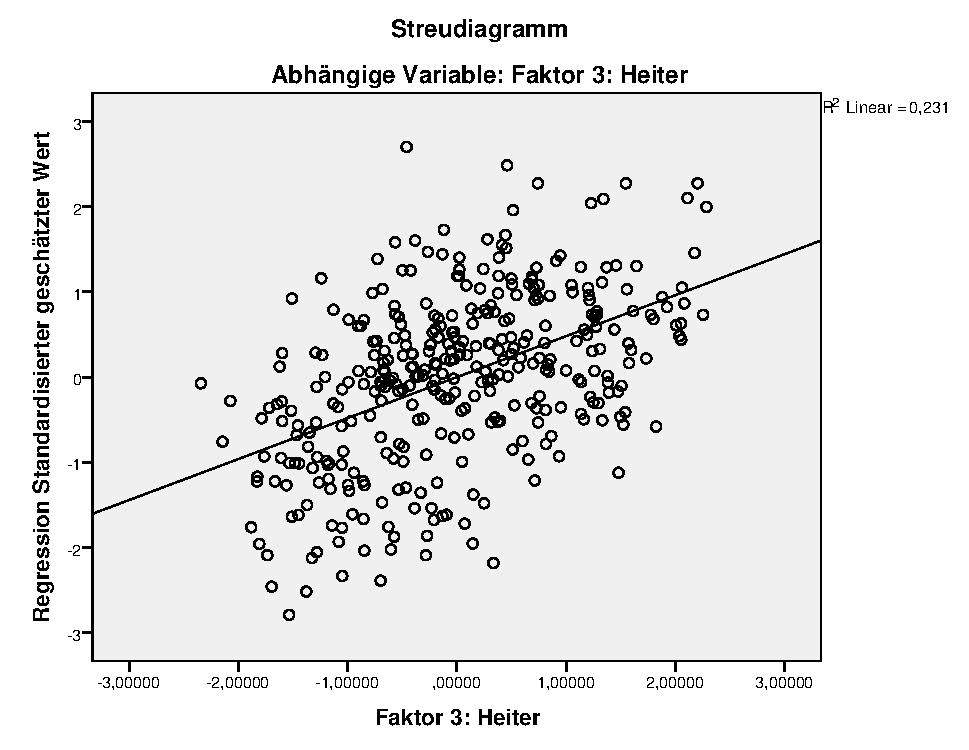
\includegraphics[width=8cm]{images/StreudiagrammFak3.pdf}
    \end{center}
    \caption{Streudiagramm und Regressionsgerade der Regression mit dem Faktor \textit{Heiter}. Diese liefert die beste Modellanpassung.}
    \label{fig:Faktor3}
\end{figure}

\section*{Diskussion}
\label{sec:Diskussion}


Die Modelle der Regressionen sind hochsignifikant.
Somit ist ein Zusammenhang zwischen den Bewertungen der Probanden und den Features von Spotify vorhanden.
Die Effektstärken der Modelle sind dagegen eher gering. 
Der höchste Korrelationskoeffizient von 0,481 ist bei der Regression mit dem Faktor \textit{Heiter} vorzufinden. Die weiteren drei Regressionen liefern noch kleinere Korrelationswerte.
Die Deutung der Korrelationswerte der erstellten Modelle auf die Faktoren von dem Datensatz "`10 Songs für die einsame Insel"' deckt sich auch mit der Interpretation von Effektstärken von Cohen.
Dabei entspricht der Korrelationswert r für die Regression mit dem Faktor \textit{Niveauvoll} einem kleinen Effekt, die übrigen entsprechen einem mittleren Effekt. 
Ein starker Effekt, der bei einem Korrelationswert von mindestens 0,5 vorzufinden ist, wird nicht erreicht \cite{cohen1988}.
Somit kann die in der Hypothese formulierte Annahme einer starken Korrelation der Datensätze mit einem Wert von mindestens 0,5 nicht bestätigt werden. 

Die Ergebnisse zeigen, dass die MIR Verfahren von Spotify zur Bewertung von Musikstücken noch Verbesserungspotential haben.
Jedoch sind auch beim Datensatz "`10 Songs für die einsame Insel"' Fehler zu erwarten, die in einen kleineren Korrelationskoeffizienten resultieren könnten.
Die Songs wurden jeweils nur einmal von nur einer Person bewertet.
Hinzu kommt, dass die Probanden einen besonderen, persönlichen Bezug zu den von ihnen bewerteten Musikstücken haben.
Eine höhere Anzahl an Bewertungen eines einzelnen Musikstücks durch mehrere Probanden mit anschließender Mittelung würden die in diesem Datensatz vorhandenen Fehler minimieren.

Ein weiterer Grund für die geringe Korrelation könnte aber auch die inhaltlich meist nicht direkt entsprechenden Bewertungskriterien beider Datensätze sein.
Es gibt beispielsweise für den Faktor, mit dem schwächsten Korrelationswert, \textit{Niveauvoll} kein Spotify Feature, das diesem Faktor inhaltlich zugeordnet werden kann.
Dahingegen lässt sich eine starke negative Korrelation des Spotify Features \textit{SP\_energy} mit dem Faktor \textit{Ruhig} inhaltlich sinnvoll erschließen.
Gleiches gilt auch für die Korrelation der Features \textit{SP\_danceability}, \textit{SP\_energy}, \textit{SP\_instrumentalness} und \textit{SP\_valence} mit dem Faktor \textit{Heiter}.
Jedoch wurde eine größere Abhängigkeit dieser inhaltlich ähnlichen Variablen, vor allem \textit{SP\_danceability} und \textit{SP\_valence} mit dem Faktor \textit{Heiter} erwartet.
Die Spotify Features \textit{SP\_tempo}, \textit{SP\_liveness}, sowie \textit{SP\_acousticness} korrelieren dagegen nicht signifikant mit einem der Faktoren und werden in keinem Modell aufgenommen. 
Das Feature \textit{SP\_tempo} beschreibt, wie die schon im vorhinein von der Analyse nicht berücksichtigten Features von Spotify, eher die Struktur eines Musikstücks und ähnelt inhaltlich somit keinem der subjektiver Empfindungen entsprechenden Bewertungen aus dem Datensatz "`10 Songs für die einsame Insel"'.
\textit{SP\_liveness} und \textit{SP\_acousticness} entsprechen inhaltlich ebenfalls keinem der "`Insel"'-Variablen.  

Eine neue empirische Studie, bei der die in dem Datensatz "`10 Songs für die einsame Insel"' vorzufindenden Bewertungskriterien für Musikstücke durch die Spotify Features ersetzt werden würde damit zu einem aussagekräftigerem Ergebnis führen.




\section*{Danksagung}
\label{sec:Danksagung}
Besonderen Dank gilt Herrn Martin Gempel, dem Autor der ursprünglich "`10 Songs für die einsame Insel"' Studie, dessen Datensatz wir freundlicherweise zur Verfügung gestellt bekommen haben, sowie den Studierenden der TU Berlin für ihre Teilnahme an der Studie.
Das Paper zur ursprünglichen Studie ist leider noch nicht veröffentlicht.
Ebenfalls möchten wir uns besonders  bei Herrn Prof. Dr. Stefan Weinzierl und Herrn Dr. Jochen Steffens für die Betreuung dieser Arbeit und die hilfreichen Diskussionen bedanken.


\bibliography{literatur}
\bibliographystyle{ieeetr}

\vfill%\vspace{10pt}
\hfill\date{\today}
%$\overline{\text{}}$

\end{document}
